\documentclass[conference,a4paper]{IEEEtran}

\usepackage{amsmath,amssymb,amsfonts}
\usepackage{graphicx}
\usepackage{textcomp}
\usepackage{xcolor}
\usepackage{booktabs}
\usepackage{array}
\usepackage{listings}
\usepackage{url}
\usepackage{hyperref}
\usepackage{cite}

\lstset{
	basicstyle=\ttfamily\footnotesize,
	keywordstyle=\color{blue}\bfseries,
	commentstyle=\color{gray}\itshape,
	stringstyle=\color{red},
	numbers=left,
	numberstyle=\tiny\color{gray},
	numbersep=5pt,
	frame=single,
	breaklines=true,
	captionpos=b,
	tabsize=4
}

\begin{document}

\title{Virtual Machines vs.\ Containers: Measuring Size, Startup Time, Memory and Throughput of the Same Web API on One Host\\
	{\footnotesize SEN421 --- Cloud Architecture and Services, Course Project, Fall 2026\\
		Istanbul Ayd\i n University}
}

\author{\IEEEauthorblockN{Soner Yan\i k}
	\IEEEauthorblockA{\textit{Department of Computer Engineering}\\
		\textit{Istanbul Ayd\i n University}\\
		Istanbul, Turkey \\
		Student ID: B2305.010151 \\
		soneryanik@stu.aydin.edu.tr}
}

\maketitle

\begin{abstract}
This project addresses Topic 2 of Part A and asks how much smaller, faster to start, lighter in memory and faster under load a container is than a virtual machine running exactly the same web application, and why. A small Flask API served by gunicorn was deployed on one Windows laptop in two ways: in a VirtualBox virtual machine running Ubuntu 22.04 with its own kernel, and in a Docker container that shares the kernel of the Docker Desktop host. Both received two processor cores and two gigabytes of memory. Image size, startup time, memory and throughput with the k6 load tool were measured with repeated runs, and a control container with the same libraries as the virtual machine separated the effect of virtualization from that of software versions. The container started in about half a second against thirty seconds for the virtual machine, and eight of thirteen virtual machine boots hung under the nested hypervisor setup. The container image was about thirteen times smaller, its idle memory five times lower than the memory used inside the guest, and it served two to three times more requests per second. The experiments cost nothing because they ran locally, and a cloud cost model shows that running eight services as containers on one larger machine is about forty percent cheaper than one small virtual machine per service. Containers are the better choice for fast scaling and dense packing, while virtual machines remain preferable for strong kernel level isolation.
\end{abstract}

\begin{IEEEkeywords}
cloud computing, virtualization, containers, hypervisor, performance evaluation
\end{IEEEkeywords}

\section{Introduction}
\label{sec:introduction}

Every cloud workload has to be isolated from its neighbours, and the two dominant ways of doing so are hardware virtualization, where each workload gets a virtual machine (VM) with its own operating system kernel, and operating-system-level virtualization, where workloads run as containers that share the host kernel. The choice affects how quickly a service can scale out, how many services fit on one server and therefore what the organization pays, and how strongly tenants are separated from each other.

I chose this topic because I am interested in performance in engineering systems, and the VM versus container question is a concrete case where an architectural decision has a measurable performance cost. Before running any experiment I expected containers to be roughly ten times faster than VMs and to use at least half as much memory. This paper tests that expectation.

\textbf{Question.} \emph{For the same small web API on the same host and with the same resource limits, how do a container and a VM differ in image size, startup time, memory use and requests per second, and how can these differences be explained by the hypervisor and the shared kernel?}

\textbf{Approach.} One Flask API was deployed in a VirtualBox VM and in a Docker container on a single laptop. Four metrics were measured with repeated, scripted runs. When the first results showed a large CPU gap, a control container with the VM's exact userland was added to test whether library versions, and not virtualization, caused the gap.

Section~\ref{sec:related_work} reviews the background, Section~\ref{sec:design} presents the design, Section~\ref{sec:methodology} the method, Section~\ref{sec:results} the results, Section~\ref{sec:discussion} the discussion and Section~\ref{sec:conclusion} concludes.

\section{Background and Related Work}
\label{sec:related_work}

\textbf{Hypervisors.} A hypervisor (virtual machine monitor) multiplexes the hardware between several VMs, each of which believes it owns a complete machine; Popek and Goldberg stated the classic requirements for such efficient virtualization~\cite{popek}. Type-1 hypervisors (for example Hyper-V or KVM) run directly on the hardware, whereas Type-2 hypervisors such as VirtualBox run as an application on a host operating system~\cite{west}. A VM must boot a full guest kernel and init system, and it is given a fixed block of memory. Virtualization is the foundation of the resource pooling and rapid elasticity characteristics in the NIST definition of cloud computing~\cite{nist}.

\textbf{Containers.} A container is a set of ordinary processes that the host kernel isolates with namespaces (process, network, mount views) and limits with control groups (cgroups)~\cite{dockercontainer}, \cite{dockerlimits}. There is no guest kernel to boot, so starting a container means starting a process, and memory is consumed only for what the processes actually use. The price is a weaker isolation boundary: all containers trust the same kernel~\cite{dockersec}.

\textbf{Windows specifics.} On Windows, Docker Desktop runs Linux containers inside the WSL2 utility VM, a lightweight Hyper-V VM with a real Linux kernel~\cite{wsl}, \cite{dockerwsl}. When Hyper-V is active it owns the processor's VT-x extensions, and VirtualBox must then run its VMs through the Windows Hypervisor Platform API instead of its own kernel driver~\cite{vboxman}. This layering turned out to be central to my results.

\textbf{Related studies.} Felter et al.\ compared KVM and Docker on Linux servers and found that containers match or exceed VM performance in almost all cases, with the VM overhead concentrated in I/O and the container overhead in Docker's NAT networking~\cite{felter}. Morabito et al.\ reached similar conclusions for compute, memory, disk and network benchmarks~\cite{morabito}. Both studies used bare-metal Linux hosts and a Type-1 hypervisor. My work differs in three ways: it measures startup time and memory footprint end to end for a real web service, it uses a Type-2 hypervisor in a nested configuration that is common on student and developer laptops, and it includes a control experiment that removes the software-version difference between the two alternatives.

\section{System Design}
\label{sec:design}

\subsection{Architecture}

Fig.~\ref{fig:architecture} shows the setup. The application is a 60-line Flask API with three endpoints: \texttt{/health} (readiness probe), \texttt{/hello} (a small JSON reply that stresses per-request overhead) and \texttt{/compute} (20{,}000 SHA-256 rounds per request, a CPU-bound task). In both alternatives it is served by gunicorn with two worker processes. The load generator and the measurement script run on the Windows host and reach each alternative through a port forward bound to the loopback address.

\begin{figure}[htbp]
	\centerline{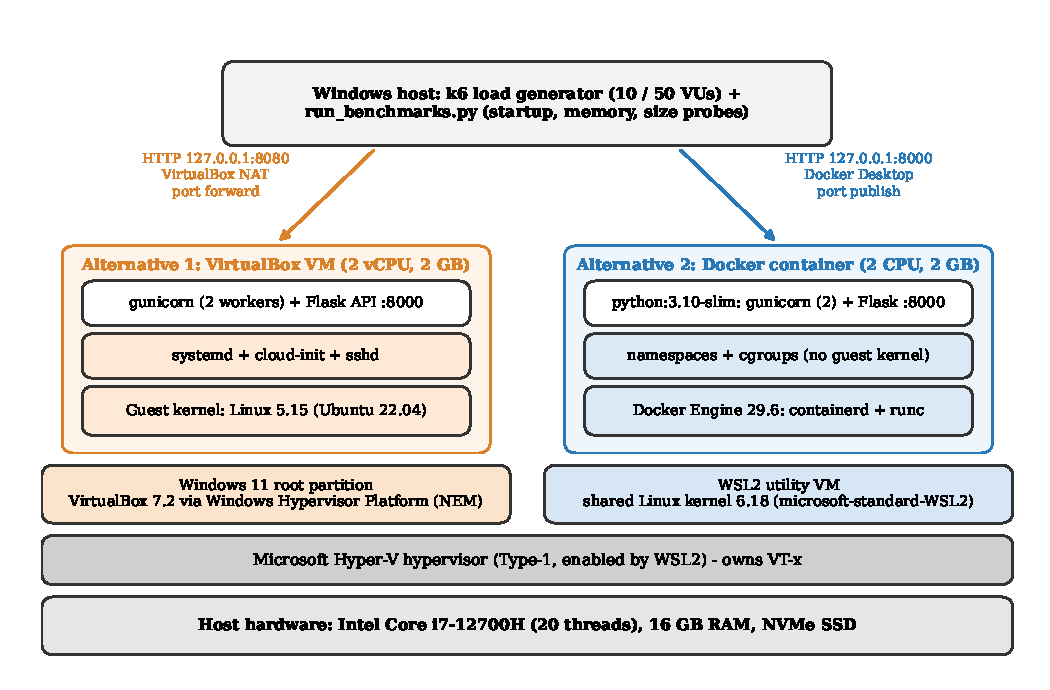
\includegraphics[width=\columnwidth]{figures/fig_architecture.pdf}}
	\caption{Architecture of the experiment. Both alternatives ultimately run on the Hyper-V hypervisor: the VM through VirtualBox and the Windows Hypervisor Platform (NEM), the container inside the WSL2 utility VM.}
	\label{fig:architecture}
\end{figure}

\subsection{Alternatives Compared}

No cloud provider was used: the topic can be completed locally~\cite{nist}, and keeping both alternatives on the same physical machine removes the run-to-run variation of shared cloud hosts.
\begin{itemize}
	\item \textbf{VM:} VirtualBox 7.2.22 running the official Ubuntu 22.04 cloud image (kernel 5.15, Python 3.10.12, OpenSSL 3.0.2), configured automatically by cloud-init; 2 vCPU, 2 GB RAM, NAT network. The API runs as a systemd service.
	\item \textbf{Container (slim):} Docker Engine 29.6.1 on the WSL2 kernel 6.18, image based on \texttt{python:3.10-slim} (Python 3.10.22, OpenSSL 3.5.7), limited with \texttt{--cpus 2 --memory 2g}.
	\item \textbf{Container (jammy), control:} the same application on \texttt{ubuntu:22.04}, which gives exactly the VM's Python and OpenSSL versions. It was added after the first results (Section~\ref{sec:results}).
\end{itemize}

\subsection{Requirements and Responsibilities}

The service must answer HTTP requests with low latency, start quickly so that it can be scaled out, and isolate the application from other workloads. Only synthetic data is processed, so no personal data under KVKK is involved. In this local setup I am responsible for every layer. In a cloud deployment the split would differ: with an IaaS VM the provider secures the hardware and hypervisor while the customer patches the guest OS, the runtime and the application; with containers on a managed container service the provider also secures the host kernel and the container runtime, and the customer remains responsible for the image contents, its vulnerabilities, secrets and network exposure~\cite{west}.

\section{Methodology}
\label{sec:methodology}

\subsection{Environment}

Table~\ref{tab:environment} lists the test environment. Only one alternative was running at a time; the other was powered off or removed so that they never competed for the host.

\begin{table}[htbp]
	\caption{Experimental Environment}
	\begin{center}
		\footnotesize
		\begin{tabular}{|l|p{0.58\columnwidth}|}
			\hline
			\textbf{Property} & \textbf{Value} \\
			\hline
			Host & Laptop, Intel Core i7-12700H (20 threads), 16 GB RAM, NVMe SSD, Windows 11 (build 26300) \\
			\hline
			Hypervisors & Hyper-V (active through WSL2); VirtualBox 7.2.22 in NEM mode \\
			\hline
			Resources & 2 vCPU and 2 GB RAM for every alternative \\
			\hline
			Application & Flask 3.0.3 API, gunicorn 22.0.0, 2 workers \\
			\hline
			Load tool & k6 v2.4.0, constant 50 and 10 virtual users (VUs) \\
			\hline
			Test duration & 10 s warm-up, then 30 s per recorded run \\
			\hline
			Repetitions & 5 successful starts; 3 load runs per endpoint, VU level and alternative; 3 runs per memory snapshot \\
			\hline
			Date & 22 November 2026 \\
			\hline
		\end{tabular}
		\label{tab:environment}
	\end{center}
\end{table}

\subsection{Measurements}

All measurements are taken by a Python script (\texttt{run\_benchmarks.py}) so that every repetition is identical:
\begin{itemize}
	\item \textbf{Image size (MiB):} Docker's disk usage and compressed content size of the image; for the VM, the size of the disk file after setup and of the downloaded cloud image.
	\item \textbf{Startup time (s):} from issuing the start command (\texttt{docker run} or \texttt{VBoxManage startvm}) until \texttt{/health} first returns HTTP 200, polled every 20 ms (container) or 100 ms (VM). The VM is shut down cleanly before each run, so every run is a cold boot. A boot that does not answer within 120 s is recorded as a hang, the VM is powered off and the run is repeated until five boots succeed.
	\item \textbf{Memory (MiB):} for the container, the cgroup usage reported by \texttt{docker stats}; for the VM, the memory used inside the guest (\texttt{free}, excluding page cache), the resident memory of the gunicorn processes, and the working set and private bytes of the VirtualBox process on Windows. Snapshots were taken while idle and 15 s into each load run.
	\item \textbf{Throughput and latency:} requests per second, median and 95th-percentile (p95) latency and error rate from k6. For runs with errors I also report \emph{goodput}, the rate of successful requests.
	\item \textbf{Pure CPU microbenchmark (s):} 200{,}000 SHA-256 rounds in one Python process, without HTTP, to isolate CPU overhead from the network path.
\end{itemize}
Means are reported with the sample standard deviation ($\pm$). Cost was tracked by keeping everything local; the cloud cost model uses Azure's official Retail Prices API~\cite{azureprices}.

\subsection{Reproducibility}

The repository listed in the Appendix contains the application, both Dockerfiles, the cloud-init template and VM creation script, the k6 test, all measurement scripts, every raw k6 summary and the CSV files behind each table and figure. The VM is reached with a locally generated SSH key that is not part of the repository; password login is disabled.

\section{Results}
\label{sec:results}

\subsection{Image Size}

The container image occupies 202~MB on disk and 49~MB compressed, of which 43~MiB is the Python base image. The VM's disk file grew to 2{,}724~MiB after setup (from a 666~MiB download), about 13 times larger in both the stored and the transferred form. The difference is the guest kernel, systemd, snap packages and a full Ubuntu userland, none of which a container needs.

\subsection{Startup Time}

Fig.~\ref{fig:startup} shows the startup times on a logarithmic axis. The slim container answered after $0.51 \pm 0.18$~s; the first run was a cold 0.83~s and the others about 0.43~s. The jammy container needed $0.38 \pm 0.02$~s. Successful VM boots needed $29.97 \pm 1.71$~s, roughly 60 to 80 times longer. Inside the guest, \texttt{systemd-analyze} showed that the kernel itself boots in about 7~s and the rest is the user space, including cloud-init and network configuration.

More important for operations, \textbf{8 of 13 VM boot attempts hung} (62\%). In each case the guest kernel stopped about 6~s into the boot while the VirtualBox process kept one host core at 100\%, and the VirtualBox log showed that it had fallen back from VT-x to the Windows Hypervisor Platform (NEM). None of the 10 container starts failed.

\begin{figure}[htbp]
	\centerline{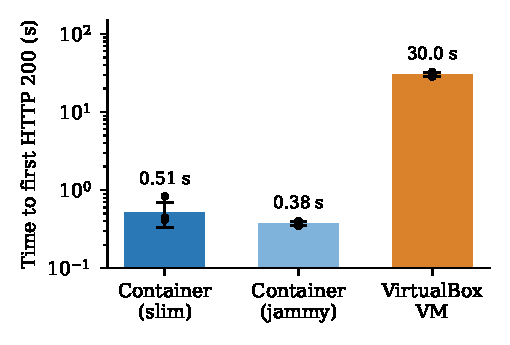
\includegraphics[width=\columnwidth]{figures/fig_startup.pdf}}
	\caption{Startup time from start command to first HTTP 200 (mean, standard deviation and individual runs; logarithmic axis). Only the 5 successful VM boots are shown; 8 further attempts hung.}
	\label{fig:startup}
\end{figure}

\subsection{Memory}

Fig.~\ref{fig:memory} compares the idle memory footprints. The container's cgroup used $43.1$~MiB idle and about 49~MiB under load. Inside the VM, the guest used $234 \pm 1$~MiB, of which only 76~MiB was the application itself; the remaining 158~MiB is the guest operating system. On the host, however, the VirtualBox process held $2{,}133$~MiB of private memory from the moment it started, because the full 2~GB of guest RAM is allocated in advance, and its working set was 755~MiB idle and up to 1{,}023~MiB under load.

A fair comparison must also account for the WSL2 utility VM that hosts every container: its process (\texttt{vmmemWSL}) had a working set of 1{,}385~MiB during the test. This is a fixed cost shared by all containers on the host (including four unrelated containers of mine that were running), while each additional container adds only about 45~MiB.

\begin{figure}[htbp]
	\centerline{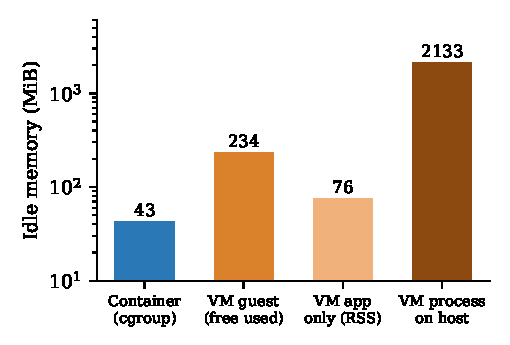
\includegraphics[width=\columnwidth]{figures/fig_memory.pdf}}
	\caption{Idle memory (logarithmic axis): container cgroup usage, memory used inside the VM guest, the application's share of it, and private memory of the VM process on the host.}
	\label{fig:memory}
\end{figure}

\subsection{Throughput and Latency}

Table~\ref{tab:throughput} summarizes the load tests, and Fig.~\ref{fig:throughput} shows the error-free runs at 10~VUs.

At 10~VUs no alternative produced any errors. The VM served $966 \pm 6$~requests/s on \texttt{/hello}, half of the container's $1{,}938 \pm 93$, and $79.8 \pm 0.5$ requests/s on \texttt{/compute}, against $208 \pm 4$ for the slim container and $237 \pm 3$ for the jammy container. The VM's p95 latency was 2.7 times higher on both endpoints.

At 50~VUs the VM's \texttt{/hello} test broke down: 81\% and 63\% of requests failed in the first two runs (0.5\% in the third), all as refused or reset connections. The raw rate of $2{,}121$~requests/s is therefore misleading; the goodput was only $746 \pm 194$~requests/s. Because the same VM served 966~requests/s without errors at 10~VUs, the failures come from the VirtualBox NAT port forward, which could not handle 50 concurrent connections, and not from the application. The containers had no errors at either load level.

\begin{table}[htbp]
	\caption{Throughput, Latency and Errors (Mean $\pm$ SD, 3 Runs)}
	\begin{center}
		\footnotesize
		\setlength{\tabcolsep}{3pt}
		\begin{tabular}{|l|c|c|c|c|}
			\hline
			\textbf{Alternative / endpoint} & \textbf{VUs} & \textbf{Goodput (req/s)} & \textbf{p95 (ms)} & \textbf{Errors} \\
			\hline
			Container slim \texttt{/hello} & 10 & $1938 \pm 93$ & $5.9$ & 0\% \\
			Container jammy \texttt{/hello} & 10 & $1945 \pm 83$ & $6.0$ & 0\% \\
			VM \texttt{/hello} & 10 & $966 \pm 6$ & $16.1$ & 0\% \\
			\hline
			Container slim \texttt{/compute} & 10 & $208 \pm 4$ & $51.5$ & 0\% \\
			Container jammy \texttt{/compute} & 10 & $237 \pm 3$ & $46.2$ & 0\% \\
			VM \texttt{/compute} & 10 & $79.8 \pm 0.5$ & $141.8$ & 0\% \\
			\hline
			Container slim \texttt{/hello} & 50 & $1888 \pm 97$ & $35.0$ & 0\% \\
			VM \texttt{/hello} & 50 & $746 \pm 194$ & $62.0$ & 48\% \\
			Container slim \texttt{/compute} & 50 & $210 \pm 4$ & $249.8$ & 0\% \\
			VM \texttt{/compute} & 50 & $78.4 \pm 2.2$ & $744.6$ & 2.4\% \\
			\hline
		\end{tabular}
		\label{tab:throughput}
	\end{center}
\end{table}

\begin{figure}[htbp]
	\centerline{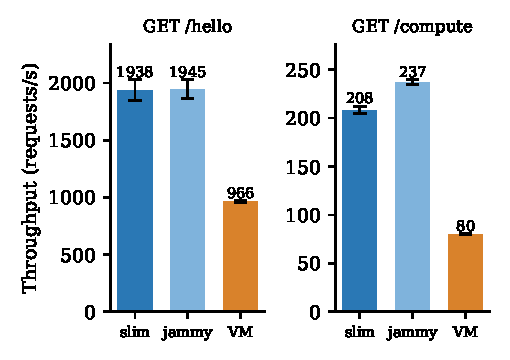
\includegraphics[width=\columnwidth]{figures/fig_throughput.pdf}}
	\caption{Throughput at 10 VUs, where no alternative had errors (mean and standard deviation of 3 runs).}
	\label{fig:throughput}
\end{figure}

\subsection{Explaining the CPU Gap: a Control Experiment}

The \texttt{/compute} gap of 2.6 times was larger than the literature suggests for CPU-bound work~\cite{felter}, \cite{morabito}. Both guests saw the same CPU model with the \texttt{sha\_ni} and \texttt{avx2} extensions, but the VM used OpenSSL 3.0.2 and the slim container OpenSSL 3.5.7. My hypothesis was that the older library, not virtualization, caused the gap. The jammy control container, with exactly the VM's Python 3.10.12 and OpenSSL 3.0.2, rejected this hypothesis: it was even slightly faster than the slim container (237 vs.\ 208~requests/s). The pure CPU microbenchmark confirms it: 200{,}000 hash rounds took $0.079 \pm 0.001$~s in the slim container, $0.079 \pm 0.002$~s in the jammy container and $0.27 \pm 0.11$~s in the VM (best run 0.20~s). The VM's CPU penalty is therefore caused by the virtualization path, not by the software inside it, and it is also much more variable.

\subsection{Cost Results}

The actual cost of all experiments was \textbf{0~USD}: everything ran on my own laptop and no cloud account was used, so no billable resources were ever created (Section~\ref{sec:conclusion}).

To translate the measurements into cloud cost, I modelled a team that must run eight small, isolated API services (for example one per customer). Prices are Azure pay-as-you-go Linux prices for the Germany West Central region, read from the Azure Retail Prices API~\cite{azureprices} on 22 November 2026, with 730 hours per month; disks, traffic and support are excluded. \emph{Option VM:} one B2s VM (2 vCPU, 4 GiB) per service, \$0.048/h. \emph{Option container:} all eight services as containers on one D4s\_v5 VM (4 vCPU, 16 GiB), \$0.23/h. Measured memory makes this feasible: eight containers need about 8~$\times$~49~MiB~$\approx$~0.4~GiB plus the host OS. Table~\ref{tab:cost} shows that the container option is about 40\% cheaper. Memory alone would allow far denser packing: with 14~GiB usable, about six 2~GiB VMs but roughly 290 containers of 49~MiB would fit, so CPU, not memory, becomes the limit for containers.

\begin{table}[htbp]
	\caption{Monthly Cost of Eight Isolated Services (Azure, USD)}
	\begin{center}
		\footnotesize
		\begin{tabular}{|l|c|c|}
			\hline
			\textbf{Cost item} & \textbf{VM per service} & \textbf{Containers} \\
			\hline
			Machines & 8 $\times$ B2s & 1 $\times$ D4s\_v5 \\
			\hline
			Hourly price & 8 $\times$ 0.048 & 0.230 \\
			\hline
			Compute per month & 280.32 & 167.90 \\
			\hline
			Experiment cost (actual) & 0.00 & 0.00 \\
			\hline
		\end{tabular}
		\label{tab:cost}
	\end{center}
\end{table}

\subsection{Comparison of Alternatives}

Measured against my initial expectation, the container was about 60 times faster to start (I expected 10), 2 to 3 times faster under load (I expected 10), and used 5 times less memory than the VM guest and 50 times less than the VM process reserved (I expected 2). The container wins on every metric measured here; the VM's advantages lie in isolation, discussed next.

\section{Discussion}
\label{sec:discussion}

\textbf{Which alternative is better, and why?} For a stateless web API that must scale with demand, the container is clearly better. The startup result follows directly from the architecture: a container start only creates namespaces and cgroups and launches gunicorn, whereas a VM must initialise virtual firmware, boot a kernel and run systemd and cloud-init. For autoscaling this is decisive: at the measured \texttt{/compute} rate, a VM that needs 30~s to join the pool leaves about 2{,}400 requests to be absorbed by the existing instances, while a container joins in under half a second. The memory result follows from the same idea. A VM's RAM is reserved up front and the guest OS is duplicated for every instance, while containers share one kernel and consume only what their processes use.

\textbf{The hypervisor layer matters more than expected.} The large CPU penalty, the boot hangs and the NAT failures all trace back to the nested configuration in Fig.~\ref{fig:architecture}: because WSL2 activates Hyper-V, VirtualBox cannot use VT-x directly and must route its virtualization through a user-mode API, so every exit from the guest becomes more expensive. The containers were also inside a VM, the WSL2 utility VM, but that VM uses Hyper-V natively and is started once and then shared. This is close to how containers are used in the cloud, where they normally run on top of VMs, and it shows that a VM is not inherently slow: a Type-1 hypervisor on bare metal, as in the cited studies, has a much smaller CPU overhead~\cite{felter}, \cite{morabito}. My CPU and boot-reliability numbers should therefore be read as properties of this nested Type-2 setup, not of all VMs.

\textbf{What would change at scale?} The fixed cost of the WSL2 VM (about 1.4~GiB) is larger than one VirtualBox guest's working set, so for a \emph{single} instance the memory advantage of Docker Desktop is small. The advantage grows with every extra instance, because each container adds only about 45~MiB. On a Linux cloud server the fixed cost largely disappears because containers run directly on the host kernel.

\textbf{Security and shared responsibility.} The VM offers the stronger boundary: a compromised application must also escape a separate kernel and the hypervisor. All containers share one kernel, so a kernel vulnerability can affect every tenant, and isolation depends on namespaces, cgroups, capabilities and seccomp profiles~\cite{dockersec}. My own configuration also had weaknesses that I would fix before production: the container ran gunicorn as root (the VM service ran as the unprivileged \texttt{nobody} user), and \texttt{docker run -p 8000:8000} publishes the port on all host interfaces, whereas the VM's port forward was bound to 127.0.0.1 only. On the positive side, the VM accepted only SSH key authentication and no secret was placed in the repository. In the cloud, the provider would protect the physical host and hypervisor in both cases, and with a managed container service also the host kernel; the image contents, patching of the base image and network exposure would remain my responsibility. For multi-tenant systems with untrusted code, VMs or sandboxed container runtimes remain the safer choice.

\textbf{Limitations.} (i) All results come from one laptop with a nested Hyper-V and VirtualBox setup; on a Linux host with KVM the CPU gap and the boot hangs would likely shrink or disappear. (ii) The network paths differ: VirtualBox NAT versus Docker Desktop's port publishing, which limited the VM at 50~VUs. (iii) Load runs lasted 30~s and were repeated three times; longer runs would give tighter confidence intervals. (iv) The load generator ran on the same host and competed for CPU, although the host had 20 threads. (v) Four unrelated containers were running in the WSL2 VM during the tests. (vi) The cloud cost model uses list prices and ignores disks, traffic, reserved-instance discounts and the operational effort of running a container platform.

\textbf{Surprising findings.} Three results surprised me. First, the VM boot failure rate of 62\%, which would be unacceptable for an autoscaling group. Second, the VM's errors at 50~VUs came from the virtual network, not from the application. Third, my OpenSSL hypothesis was wrong, which showed me the value of a control experiment before attributing a difference to a cause.

\textbf{Legal and ethical points.} Only synthetic requests were used, no personal data was processed and all tests targeted resources I own, so KVKK obligations were not triggered. In a real deployment the choice between VMs and containers does not change data-residency obligations, but the stronger isolation of VMs can simplify demonstrating tenant separation in audits.

\section{Conclusion and Future Work}
\label{sec:conclusion}

For the same Flask API with the same 2~vCPU and 2~GB limits, the container started in 0.4 to 0.5~s instead of 30~s, its image was 13 times smaller, it used 43~MiB instead of 234~MiB inside the guest (and 2.1~GiB reserved on the host), and it served 2 to 3 times more requests per second without the errors and boot hangs observed for the VM. A control container proved that the CPU gap comes from the virtualization layer and not from library versions. I would recommend containers to an organization that runs many small, stateless services and needs fast scale-out, which in the modelled case saves about 40\% of compute cost, and VMs where strong kernel-level isolation or a different operating system is required.

The main lesson I learned is that the environment around a hypervisor can dominate its performance: the nested Hyper-V setup, not virtualization itself, produced the largest penalties. With more time I would repeat the experiment on a Linux host with KVM and on a cloud VM, measure scale-out in a real autoscaling group, test a sandboxed runtime such as gVisor or a microVM such as Firecracker, and run longer tests.

No cloud account was used, so no billable resources exist. The local VM, its disk and the container images are kept until the project has been evaluated, so that any measurement can be repeated on request, and are deleted afterwards with the cleanup commands in the repository. The VM accepts only key-based SSH on the loopback address, so keeping it creates no exposure.

\section*{AI Tool Use and Originality Declaration}
\label{sec:ai_declaration}
% NOTE (Soner): You may edit this section. Keep it truthful: if you rewrite
% parts yourself or take over tasks, lower the corresponding levels.

AI-assisted tools (Claude, Anthropic, used through Claude Code) were used extensively in this project, as summarized in Table~\ref{tab:ai_use}. The topic choice, the motivation, the initial performance expectations and the personal information were provided by the student. The AI tool proposed the experimental design, wrote the application, Dockerfiles, VM configuration and measurement scripts, ran the experiments on the student's computer, produced the figures and drafted the report text and its interpretation, which the student reviewed. All numbers in this report come from measurements actually executed on the student's laptop on 22 November 2026; the raw outputs are in the repository. Prices were taken from the official Azure Retail Prices API and references were checked against the original sources. The student accepts full responsibility for the accuracy, originality, reproducibility and integrity of the submitted work.

\begin{table}[htbp]
	\caption{AI Use Disclosure Summary}
	\label{tab:ai_use}
	\centering
	\footnotesize
	\begin{tabular}{|p{0.33\linewidth}|c|p{0.42\linewidth}|}
		\hline
		\textbf{Project Stage} & \textbf{Level} & \textbf{Brief Description} \\
		\hline
		Topic and question & 3 & Student chose the topic and motivation; AI refined the research question \\
		\hline
		Literature and documentation search & 4 & AI proposed sources and verified links; student reviewed \\
		\hline
		Design, deployment, and configuration & 5 & AI designed the setup and wrote code and configuration \\
		\hline
		Measurement, cost analysis, and modeling & 5 & AI wrote and ran the scripts on the student's machine and built the cost model \\
		\hline
		Writing, editing, and LaTeX formatting & 5 & AI drafted the report and formatted it in LaTeX \\
		\hline
		Interpretation, discussion, and conclusion & 4 & AI drafted the interpretation; student supplied motivation and expectations and reviewed it \\
		\hline
	\end{tabular}
\end{table}

\begin{thebibliography}{00}

\bibitem{nist} P.~Mell and T.~Grance, ``The NIST definition of cloud computing,'' National Institute of Standards and Technology, Gaithersburg, MD, USA, NIST Special Publication 800-145, 2011.

\bibitem{west} J.~West, \textit{CompTIA Cloud+ Guide to Cloud Computing}, 2nd~ed. Boston, MA, USA: Cengage, 2024.

\bibitem{popek} G.~J.~Popek and R.~P.~Goldberg, ``Formal requirements for virtualizable third generation architectures,'' \textit{Communications of the ACM}, vol.~17, no.~7, pp.~412--421, 1974.

\bibitem{felter} W.~Felter, A.~Ferreira, R.~Rajamony, and J.~Rubio, ``An updated performance comparison of virtual machines and Linux containers,'' in \textit{Proc. IEEE Int. Symp. Performance Analysis of Systems and Software (ISPASS)}, Philadelphia, PA, USA, 2015, pp.~171--172.

\bibitem{morabito} R.~Morabito, J.~Kj\"allman, and M.~Komu, ``Hypervisors vs. lightweight virtualization: A performance comparison,'' in \textit{Proc. IEEE Int. Conf. Cloud Engineering (IC2E)}, Tempe, AZ, USA, 2015, pp.~386--393.

\bibitem{dockercontainer} Docker Inc., ``What is a container?,'' Docker Docs. [Online]. Available: \url{https://docs.docker.com/get-started/docker-concepts/the-basics/what-is-a-container/}. [Accessed: 22 Nov. 2026].

\bibitem{dockerlimits} Docker Inc., ``Resource constraints,'' Docker Docs. [Online]. Available: \url{https://docs.docker.com/engine/containers/resource_constraints/}. [Accessed: 22 Nov. 2026].

\bibitem{dockersec} Docker Inc., ``Docker Engine security,'' Docker Docs. [Online]. Available: \url{https://docs.docker.com/engine/security/}. [Accessed: 22 Nov. 2026].

\bibitem{dockerwsl} Docker Inc., ``Docker Desktop WSL 2 backend on Windows,'' Docker Docs. [Online]. Available: \url{https://docs.docker.com/desktop/features/wsl/}. [Accessed: 22 Nov. 2026].

\bibitem{wsl} Microsoft, ``Comparing WSL versions,'' Microsoft Learn. [Online]. Available: \url{https://learn.microsoft.com/en-us/windows/wsl/compare-versions}. [Accessed: 22 Nov. 2026].

\bibitem{vboxman} Oracle, ``Chapter 10. Technical background,'' Oracle VirtualBox User Manual. [Online]. Available: \url{https://www.virtualbox.org/manual/ch10.html}. [Accessed: 22 Nov. 2026].

\bibitem{azureprices} Microsoft, ``Azure Retail Prices REST API overview,'' Microsoft Learn. [Online]. Available: \url{https://learn.microsoft.com/en-us/rest/api/cost-management/retail-prices/azure-retail-prices}. [Accessed: 22 Nov. 2026].

\bibitem{k6} Grafana Labs, ``Grafana k6 documentation.'' [Online]. Available: \url{https://grafana.com/docs/k6/latest/}. [Accessed: 22 Nov. 2026].

\end{thebibliography}

\appendix

\section{Code Repository}
\label{app:code}

Application, configuration, scripts and raw results: \url{https://github.com/soneryanik/cloud-vm-container-test}. The load test is run with k6~\cite{k6}; the core of the startup measurement is:

\begin{lstlisting}[language=Python, caption={Startup time measurement (excerpt of run\_benchmarks.py)}, label={lst:startup}]
t0 = time.perf_counter()
vm_start()          # or container_start()
t_cmd = time.perf_counter() - t0
try:
    t_ready = t_cmd + wait_http(
        "http://127.0.0.1:8080/health", 120, 0.1)
    status = "ok"
except TimeoutError:   # boot hung
    t_ready, status = "", "hang"
    vm_hard_off()
\end{lstlisting}

\section{Deployment Evidence}
\label{app:evidence}

Fig.~\ref{fig:evidence} shows two console screenshots of the VM taken with \texttt{VBoxManage controlvm screenshotpng}: a successful boot reaching the login prompt, and one of the hung boots, stopped after the network driver initialised. Listing~\ref{lst:cli} shows command-line output from the measurement run, the VirtualBox log and the running guest.

\begin{figure*}[t]
	\centering
	\begin{minipage}[b]{0.3\textwidth}\centering
		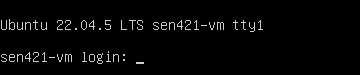
\includegraphics[width=\linewidth]{figures/vm_console_login_crop.png}\\[2pt]
		{\footnotesize (a) successful boot}
	\end{minipage}\hfill
	\begin{minipage}[b]{0.66\textwidth}\centering
		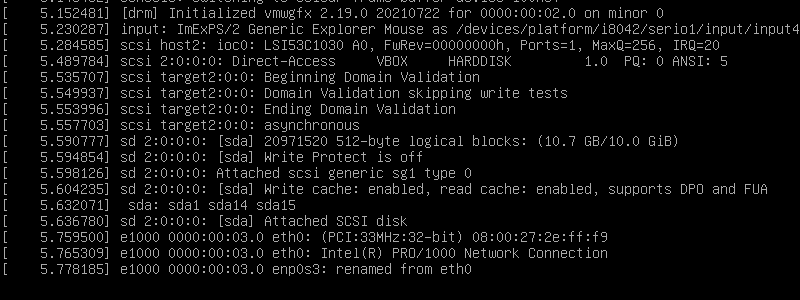
\includegraphics[width=\linewidth]{figures/vm_console_boot_hang_crop.png}\\[2pt]
		{\footnotesize (b) hung boot: the last kernel messages before the stop}
	\end{minipage}
	\caption{VM console screenshots (cropped). (a) Successful boot to the login prompt. (b) One of the hung boots; the kernel stopped at about 5.8~s after the network driver initialised.}
	\label{fig:evidence}
\end{figure*}

\begin{lstlisting}[language={}, numbers=none, basicstyle=\ttfamily\scriptsize, caption={Command-line output (excerpts; column spacing condensed to fit)}, label={lst:cli}]
# run_benchmarks.py (results/benchmark_log.txt)
[14:04:44] 2) startup time: vm x5
[14:06:57]    attempt 1: hang
[14:11:56]    attempt 4: ok, ready after 28.43 s
[14:33:29] summary
  container startup    0.51 s +- 0.18
  vm        startup   29.97 s +- 1.71

# VirtualBox log (VBox.log)
00:00:01.196216 HM: HMR3Init: Attempting fall back to NEM: VT-x is not available

# inside the VM (ssh sen421@127.0.0.1 -p 2222)
  Virtualization: oracle
Operating System: Ubuntu 22.04.5 LTS
          Kernel: Linux 5.15.0-203-generic
{"cpus":2,"host":"sen421-vm","kernel":"5.15.0-203-generic","python":"3.10.12"}

# docker images sen421-api
IMAGE            ID           DISK USAGE CONTENT SIZE
sen421-api:1.0   5d61232445ab      202MB       49.2MB
sen421-api:jammy 4e50b56b80f1      208MB       51.3MB
\end{lstlisting}

\end{document}
